% Created 2023-05-11 Thu 16:40
% Intended LaTeX compiler: pdflatex
\documentclass[9pt, b5paper]{article}
\usepackage{xeCJK}
\usepackage[T1]{fontenc}
\usepackage{bera}
\usepackage[scaled]{beraserif}
\usepackage[scaled]{berasans}
\usepackage[scaled]{beramono}
\usepackage[cache=false]{minted}
\usepackage{xltxtra}
\usepackage{graphicx}
\usepackage{xcolor}
\usepackage{multirow}
\usepackage{multicol}
\usepackage{float}
\usepackage{textcomp}
\usepackage{algorithm}
\usepackage{algorithmic}
\usepackage{latexsym}
\usepackage{natbib}
\usepackage{geometry}
\geometry{left=1.2cm,right=1.2cm,top=1.5cm,bottom=1.2cm}
\usepackage[xetex,colorlinks=true,CJKbookmarks=true,linkcolor=blue,urlcolor=blue,menucolor=blue]{hyperref}
\newminted{common-lisp}{fontsize=\footnotesize} 
\author{deepwaterooo}
\date{\today}
\title{ET 框架拖拉机项目试改装}
\hypersetup{
 pdfauthor={deepwaterooo},
 pdftitle={ET 框架拖拉机项目试改装},
 pdfkeywords={},
 pdfsubject={},
 pdfcreator={Emacs 28.2 (Org mode 9.5.5)}, 
 pdflang={English}}
\begin{document}

\maketitle
\tableofcontents


\section{双副牌双升108 张卡牌游戏}
\label{sec:org06776f0}
\begin{itemize}
\item 【游戏可试玩程序】:放在Release/Tractor.exe. Windows 用户大家可以下载试玩儿体验一下。
\item 昨天晚上找见了别人几年前就开发出来的卡五星麻将,所以写麻将游戏的想法就被恶杀在摇篮中。现在再写什么好呢?就只能写【双升拖拉机】了,就是两副牌108 张来打的拖拉机。现已经 ios iPhone 上有的双升游戏,可能搜索一下设计,写安卓版的双升了,看下能否套用ET 框架,写成四人网络【客户端与服务器双热更新的】网络游戏
\item 现在先搜索必要的框架设计,出版规则比大小算法之类的。
\item 【服务器与客户端的同步】:尤其是在分四人牌后,亮主拖底的时候,谁先亮,亮什么主,顺序重要,结果重要。【 ET 框架有专用的游戏服,由游戏服来状态同步】在本程序中,采用的是服务器保存所有的状态,处理所有的逻辑。比如,客户端在点击亮主后,做的事情就是发一个消息给服务器,不做任何显示操作,等待服务器传来亮主的消息后再显示
\begin{itemize}
\item 【发牌,公正性】:随机分牌。第一步就是要发牌。需要做到一个完全随机的发牌,就要保证每张牌发到每个玩家手里的概率都是一样的,而且牌的顺序是等概率随机打乱的。程序中采用的是如下的发牌算法(感谢Dr.Light提供):假如有两幅牌,编号从1到108,首先随机选出一个,并且将牌发给玩家,然后将这个编号的牌与108号牌交换编号,那么剩下的牌就是从1到107号。于是再从中选出一个,重复以上的过程,这样一来,算法的复杂度就是O(n)。
\end{itemize}
\item 【牌的逻辑OOD/OOP】设计:三个类,对应单张,拖拉机(对子是长度为1 的拖拉机),和混合单张与拖拉机
\item 第一手牌与非第一手牌的处理:
\end{itemize}

\begin{center}
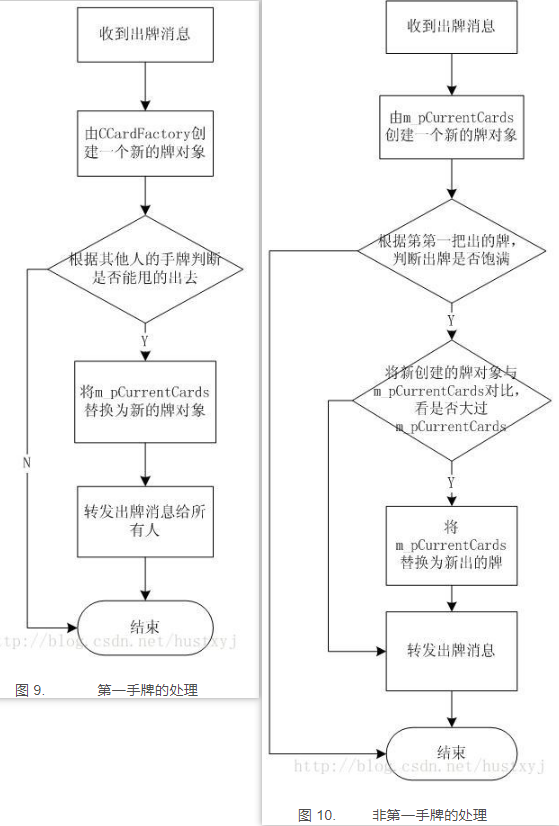
\includegraphics[width=.9\linewidth]{./pic/plan_20230508_223827.png}
\end{center}

\begin{itemize}
\item 参考一个很Q 的界面:
\end{itemize}

\begin{center}
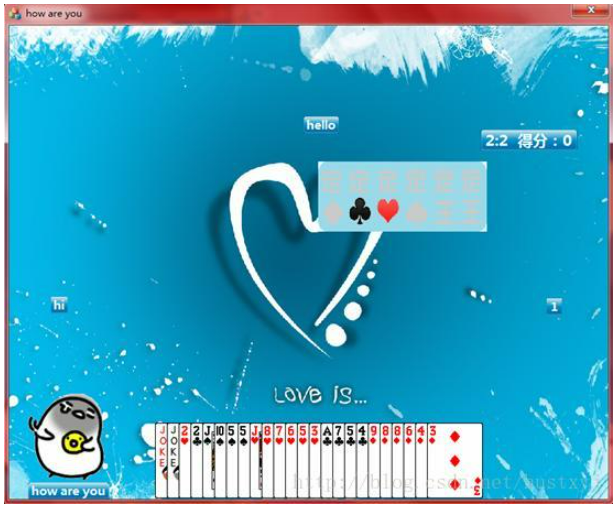
\includegraphics[width=.9\linewidth]{./pic/plan_20230508_222717.png}
\end{center}

\begin{center}
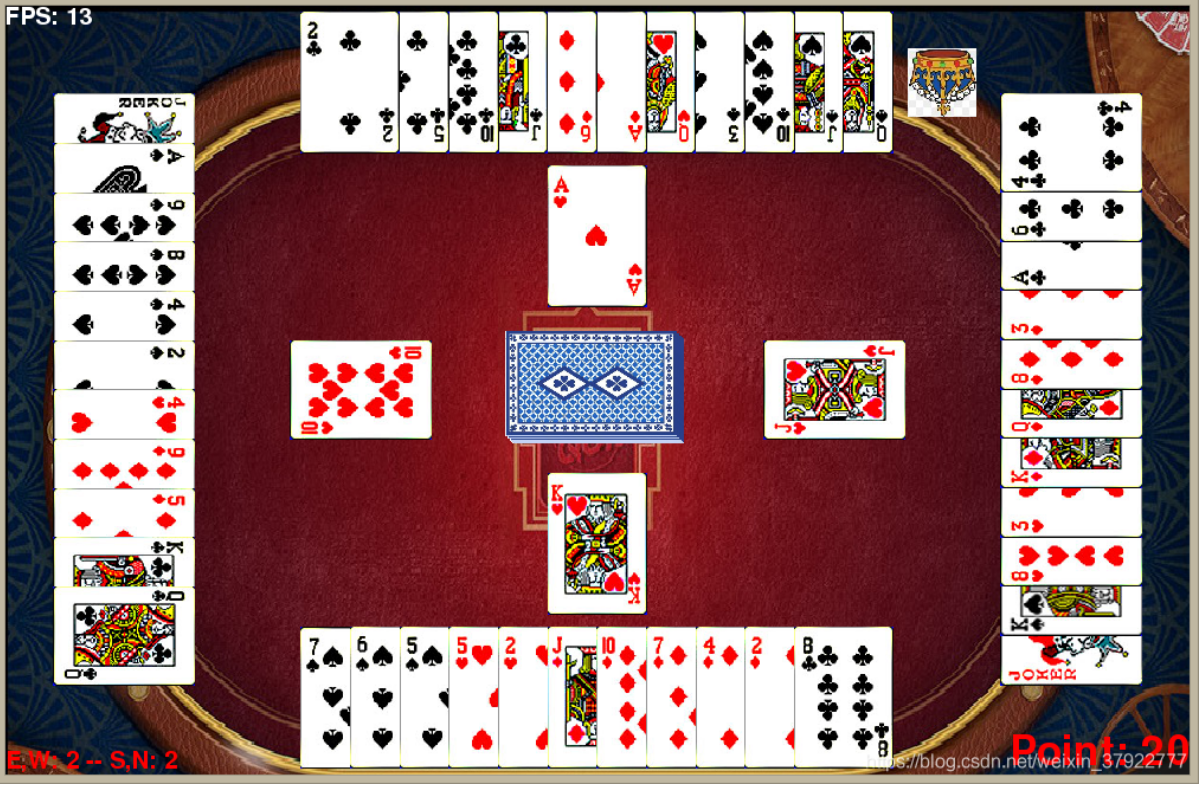
\includegraphics[width=.9\linewidth]{./pic/plan_20230508_221732.png}
\end{center}
\begin{itemize}
\item 亮着牌打的不好玩,一定会把其它三副牌藏起来的
\item \url{http://www.homygame.com/ngscom/help/shengji.htm}
\item 简易版设计原理:模拟拖拉机(升级)玩法;
\begin{itemize}
\item 1.创建两副牌的集合:HashMap
\item 2.创建纸牌:四个花色共108张♦ ♣ ♥ ♠
\item 3.创建poker的ArrayList操作集合
\item 4.创建亮主牌的操作
\item 5.将所有牌放入牌盒中
\item 6.创建四个玩家与底牌的集合:HashSet wj1,wj2,wj3,wj4,dipai
\item 7.洗牌
\item 8.发牌操作
\item 9.创建看牌方法
\item 10.调用方法看牌
\end{itemize}
\item 安桌上的游戏现在是这样的:还要再写一个吗?【活宝妹就是一定要嫁给亲爱的表哥!!!】还是说更为完善或是好玩儿的游戏逻辑?或是UI 视图画面,或是性能表现?反正一定是套用ET 框架写得最容易快速方便。【感觉现在这个截图的UI 长得有点儿丑怪。。】不好看不经典,看了就不想玩儿了。。
\end{itemize}
\section{主要参考项目:}
\label{sec:org9aee684}
\begin{itemize}
\item 【ET- 斗地主游戏】年代久远,ET 框架的版本古旧。手游风格的界面设计
\item 【ET- 卡五星游戏】年代久远,ET 框架的版本古旧。主要看牌类相关的房间内的逻辑
\item 分支 7.2 与主分支的区别:都有最开始必须取消主相机。区别是进入地图时,7.2 如果再激活相机,可以看见地图,小人也能跟随鼠标右键动。主分支可能还需要我再看一下,为什么主分支进入不了地图。两个分支对比一下,主要是让自己放心,现所使用的主分支应该没有 blocking 【BUG:】存在。去看下主分支,可以显示地图吗
\item 截几个斗地主游戏里的流程图供自己写时参考:
\end{itemize}

\begin{center}
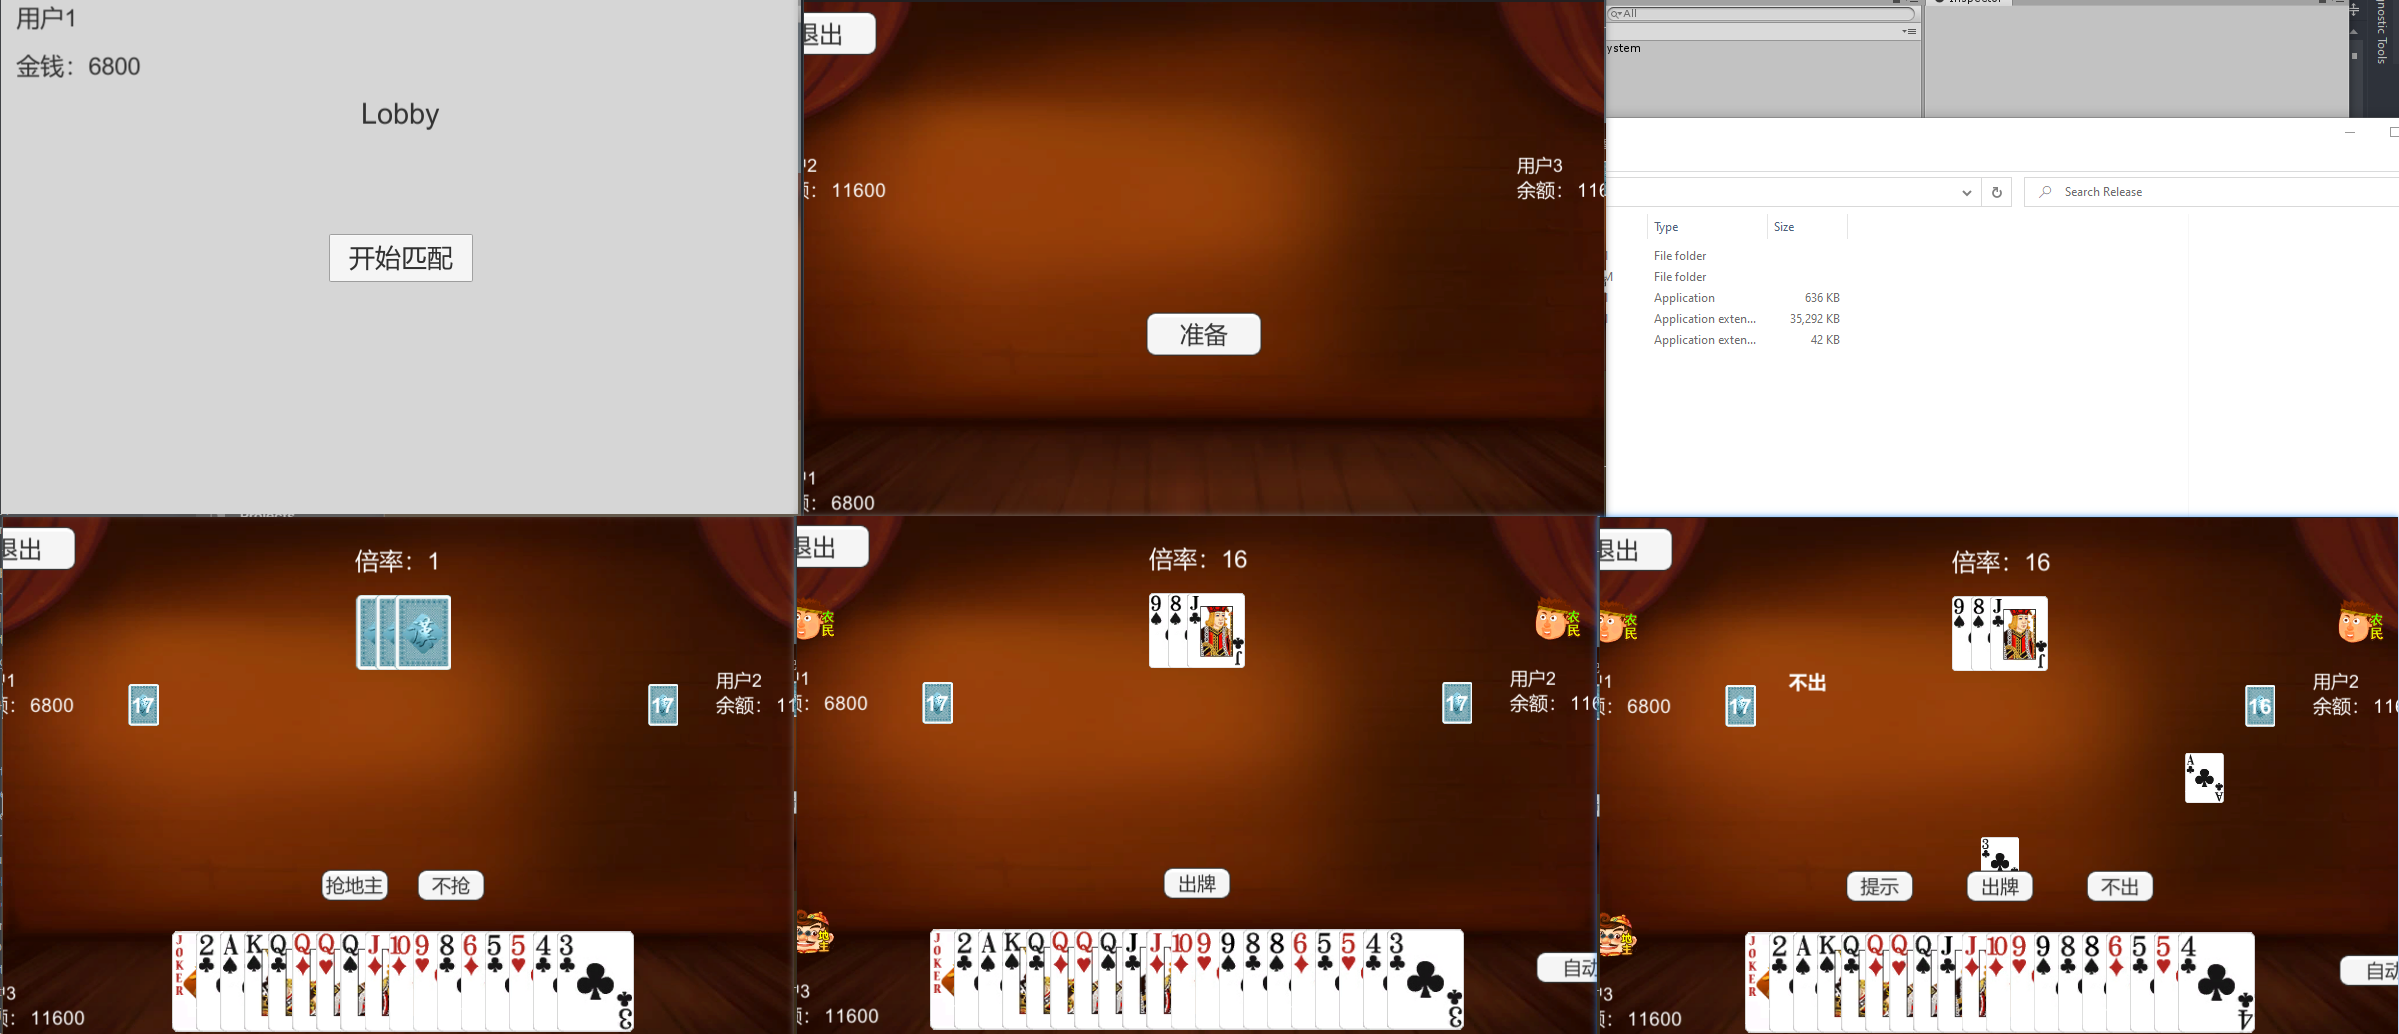
\includegraphics[width=.9\linewidth]{./pic/readme_20230511_163501.png}
\end{center}
\section{项目主要进展}
\label{sec:org04a5e04}
\begin{itemize}
\item 因为两个参考项目的版本都狠古旧,现用最新版本的ET 【我觉得这里,最好我还是先去试ET7.2 官方版本可能更好】就以自己能有的相对快速,按照现有的理解,把能重组的重组出来。不理解的,再去看下两个项目分别的实现逻辑。
\end{itemize}
\section{残余的几个小 bug}
\label{sec:orgd31139c}
\begin{itemize}
\item 当进入UILobby 的时候,要把前面的 UILogin 删除。应该是有逻辑,只是因为我现在的【BUG:】,后面就座地执行的逻辑中断了
\end{itemize}
\end{document}